\chapter{Music Theory Terms}\label{appendix:music-theory-terms}
The following list contains the definitions of frequently used musical terms in this paper. Additionally, terms which may augment the understanding of the changes made musically are included. 
\begin{itemize}
    \item {\textbf{Frequency}: the perceived pitch of a sound.}
    \item {\textbf{Volume}: the perceived loudness of a sound.}
    \item {\textbf{Timbre}: the quality of a sound, which helps to differentiate between instruments.}
    \item {\textbf{Staccato}: a directive for notes to be played detached and separated.}
    \item {\textbf{Legato}: a directive for notes to be played smoothly and connected.}
    \item {\textbf{Tie/tied notes}: for this directive, a curved line is drawn over or under the heads of notes of the same pitch. This indicates that there should be no break in the playing of these notes, and should be played as one singular note.}
    \item {\textbf{Chord}: the simultaneous sounding of two or more notes. Typically, a chord will be composed of three notes in total, created a \textit{triad}.}
    \item {\textbf{Major chord}: a chord composed of a root note (the tonic note), a major third interval above the tonic note, and a perfect fifth interval above the tonic note.}
    \item {\textbf{Tonic note}: the note of a chord or a song, which determines the key signature.}
    \item {\textbf{Key signature}: a set of sharp (\musSharp{}, or flat (\musFlat{}) symbols placed on the staff at the beginning of sheet music or a section of music.}
    \item {\textbf{Major third interval}: the interval that spans four semitones. For example, the interval between $C$ and $E$ is a major third.}
    \item {\textbf{Minor third interval}: the interval that spans three semitones. For instance, the interval between $A$ and $C$ is a minor third.}
    \item {\textbf{Texture}: how a sound is organized, and the number of layers within a sound.}
    \item {\textbf{Treble clef}: a type of musical notation to indicate the pitches represented by the lines and spaces on sheet music. Also known as the ``G-clef,'' the second line from the bottom represents the note \textit{G} above Middle C. This clef is the most common clef seen. Typically, the treble clef will contain the note Middle C, as well as notes above Middle C.}
    \item {\textbf{Alto clef}: a type of musical notation to indicate the pitches represented by the lines and spaces on sheet music. This clef is also known as the ``C-clef'' or the ``Viola clef,'' as only certain instruments, which include the viola, use this clef. The middle line of this clef represents the note Middle C.}
    \item {\textbf{Pianissimo}: a directive to perform an indicated passage of a composition or piece very softly. Abbreviated as \textit{pp}.}
    \item {\textbf{Fortissimo}: a directive to perform an indicated passage of a composition or piece very loudly. Abbreviated as \textit{ff}.}
    \item {\textbf{Interval ratio}: the ratios of the frequencies of pitches in a musical interval. As an interval is the ``distance'' between two pitches, the ratio assists musicians to work with relative pitch measures applicable to a range of instruments intuitively, rather than a set of memorized frequency values.}
    
    For instance, suppose we have a guitar as in Figure \ref{fig:guitar-math}. The \textit{interval ratio} will then be inverse to the length of the string. The total length of the string in red has a 1:1 ratio, and the remaining pitches can be described as some ratio to this total string length. On the E string of this guitar (the top string of Figure \ref{fig:guitar-math}), the note an octave above the note E is still E. Then, this note E one octave above the root note E is 12 frets above the root. As noted in the Figure, pressing down on fret 12 of the E string (or any string) results in the length of the string being halved, and an interval ratio of $\frac{1}{2}$. This produces the note one octave above the starting note.
    \item {\textbf{Equal temperament}: a system of tuning the scale, in which the octave is evenly divided into 12 equal semitones. It is based on the cycle of 12 identical fifths, or the ``circle of fifths'' \cite{Cochrane_2011}.}
    
    \begin{figure}[H]
        \centering
        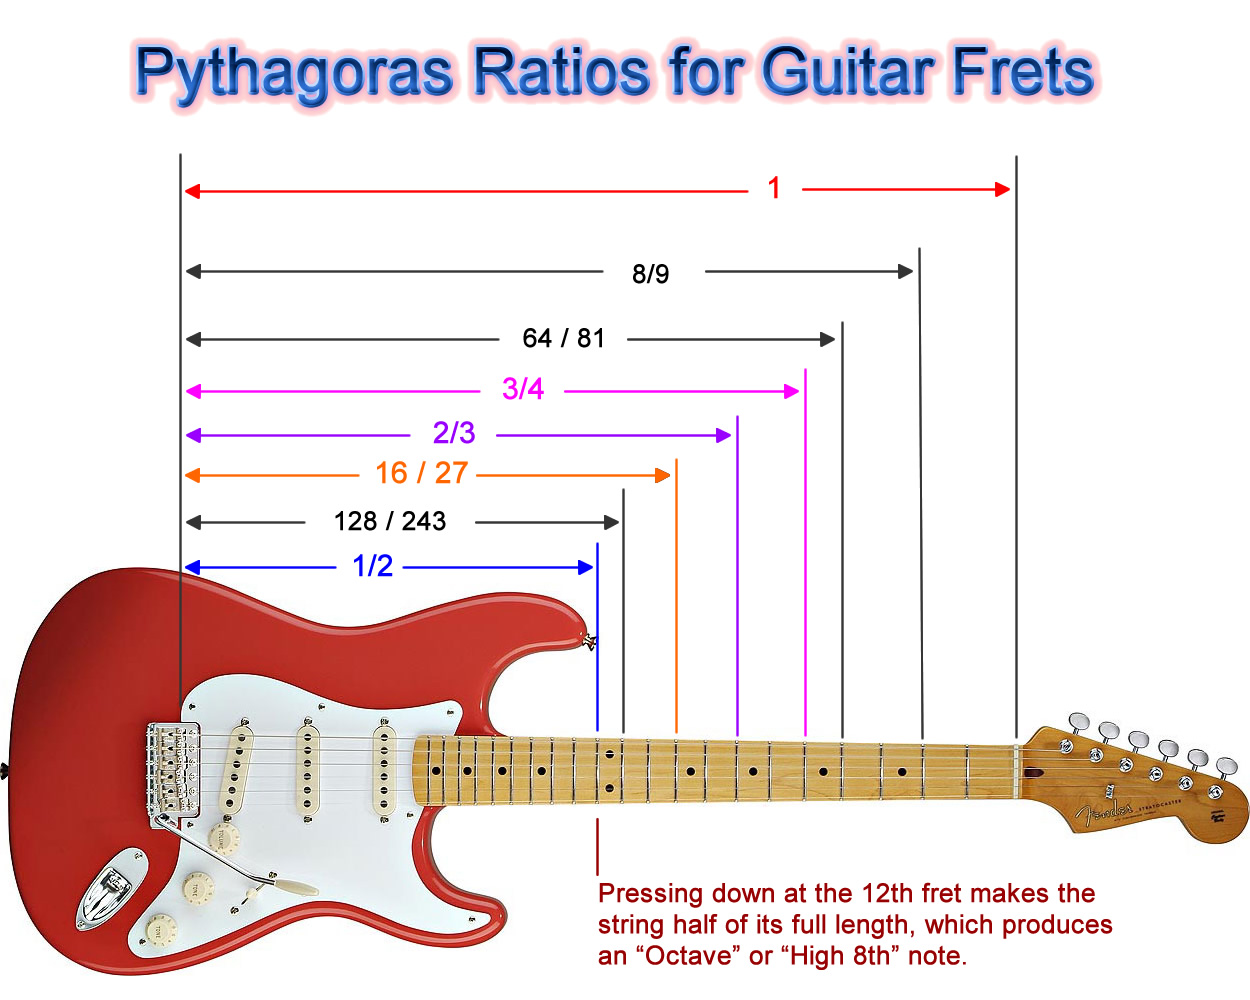
\includegraphics[width=0.4\textwidth]{figures/guitar-math.jpeg}
        \caption{Pythagoras Ratios for Guitar Frets}\cite{Passy_2012}
        \label{fig:guitar-math}
    \end{figure}
    
\end{itemize}